\documentclass[tikz,border=4pt]{standalone}
\usepackage[tt=false,type1=true]{libertine}
\usepackage[libertine]{newtxmath}
\usepackage{pgfplots}
\usetikzlibrary{patterns}
\pgfplotsset{compat=1.18}
\definecolor{budgeteight}{HTML}{0072B2}
\definecolor{budgetone}{HTML}{D55E00}
\definecolor{noservice}{HTML}{D9D9D9}
\pdfinfo{/Title (Pricing regimes as two 3D phase slices)
 /Subject (The two categorical depth slices are fixed service pricing and metered billing. No intermediate pricing modes are inferred. Qwen3.8 non-thinking, batch16, r0, model control, strict user purchase at both budgets, zero firm cost, fixed reference price and midpoint energy. The source regions and boundary ties are identical to the verified 2D example.)}
\begin{document}
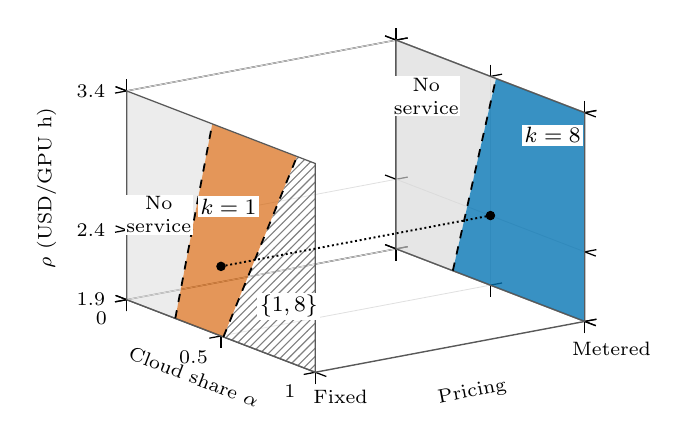
\begin{tikzpicture}
\begin{axis}[
 view={55}{23},width=7.4cm,height=5.8cm,
 xmin=0,xmax=1,ymin=0,ymax=1,zmin=1.9,zmax=3.4,
 xtick={0,.5,1},ytick={0,1},yticklabels={Fixed,Metered},
 ztick={1.9,2.4,3.4},
 tick label style={font=\fontsize{7.5}{8.5}\selectfont},
 label style={font=\fontsize{7.5}{8.5}\selectfont},
 xlabel={Cloud share $\alpha$},ylabel={Pricing},
 xlabel style={at={(xticklabel* cs:0.5,12pt)},anchor=north,sloped like x axis},
 ylabel style={at={(yticklabel* cs:0.5,12pt)},anchor=north,sloped like y axis},
 zlabel={$\rho$ (USD/GPU h)},
 grid=major,grid style={black!12,line width=.3pt},
 axis line style={black!65,line width=.5pt},
 tick style={black,line width=.45pt},
 tick align=outside,scaled ticks=false,clip=false]
% Metered slice, at categorical depth one.
\path[draw=none,fill=noservice,fill opacity=.65]
 (axis cs:0,1,1.9)--(axis cs:0.3007389129,1,1.9)--(axis cs:0.5293744961,1,3.4)--(axis cs:0,1,3.4)--cycle;
\path[draw=none,fill=budgeteight,fill opacity=.78]
 (axis cs:0.3007389129,1,1.9)--(axis cs:1,1,1.9)--(axis cs:1,1,3.4)--(axis cs:0.5293744961,1,3.4)--cycle;
\draw[black!65,line width=.45pt] (axis cs:0,1,1.9)--(axis cs:1,1,1.9)--(axis cs:1,1,3.4)--(axis cs:0,1,3.4)--cycle;
\draw[black,dashed,line width=.65pt] (axis cs:0.3007389129,1,1.9)--(axis cs:0.5293744961,1,3.4);
% Fixed-price slice, at categorical depth zero.
\path[draw=none,fill=noservice,fill opacity=.5]
 (axis cs:0,0,1.9)--(axis cs:0.2578401372,0,1.9)--(axis cs:0.4538290634,0,3.4)--(axis cs:0,0,3.4)--cycle;
\path[draw=none,fill=budgetone,fill opacity=.65]
 (axis cs:0.2578401372,0,1.9)--(axis cs:0.5130020416,0,1.9)--(axis cs:0.9030098387,0,3.4)--(axis cs:0.4538290634,0,3.4)--cycle;
\path[draw=none,fill=white,fill opacity=.3]
 (axis cs:0.5130020416,0,1.9)--(axis cs:1,0,1.9)--(axis cs:1,0,3.4)--(axis cs:0.9030098387,0,3.4)--cycle;
\path[draw=none,pattern=north east lines,pattern color=black!50]
 (axis cs:0.5130020416,0,1.9)--(axis cs:1,0,1.9)--(axis cs:1,0,3.4)--(axis cs:0.9030098387,0,3.4)--cycle;
\draw[black!65,line width=.45pt] (axis cs:0,0,1.9)--(axis cs:1,0,1.9)--(axis cs:1,0,3.4)--(axis cs:0,0,3.4)--cycle;
\draw[black,dashed,line width=.65pt] (axis cs:0.2578401372,0,1.9)--(axis cs:0.4538290634,0,3.4);
\draw[black,dashed,line width=.65pt] (axis cs:0.5130020416,0,1.9)--(axis cs:0.9030098387,0,3.4);
% Region labels and the same reference point on both slices.
\node[font=\fontsize{7.5}{8.5}\selectfont,fill=white,inner sep=.6pt,align=center] at (axis cs:.16,1,3.08) {No\\service};
\node[font=\fontsize{8}{9}\selectfont,fill=white,inner sep=1pt] at (axis cs:.83,1,3.15) {$k=8$};
\node[font=\fontsize{7.5}{8.5}\selectfont,fill=white,inner sep=.6pt,align=center] at (axis cs:.17,0,2.6) {No\\service};
\node[font=\fontsize{8}{9}\selectfont,fill=white,inner sep=1pt] at (axis cs:.54,0,2.85) {$k=1$};
\node[font=\fontsize{8}{9}\selectfont,fill=white,inner sep=1pt] at (axis cs:.86,0,2.3) {$\{1,8\}$};
\draw[black,densely dotted,line width=.7pt] (axis cs:.5,0,2.4)--(axis cs:.5,1,2.4);
\addplot3[only marks,mark=*,mark size=1.5pt,black] coordinates {(.5,0,2.4)(.5,1,2.4)};
\end{axis}
\end{tikzpicture}
\end{document}
